\section{Experiments}
\label{sec:exp}

To evaluate the versatility of DynaDebate, we conducted experiments on three backbone models: the proprietary model GPT-4o-mini and the open-source models Qwen3-8B and Llama-3.3-70B-Instruct. To facilitate a fair comparison with existing MAD methods, we standardized the multi-agent configuration to involve three agents engaging in two rounds of debate. Detailed prompts are provided in Appendix~\ref{app:prompts}.

\subsection{Experimental Setup}
\label{sec:setup}

We report results on five benchmarks in the main table; GSM8K and Biography results appear in appendices due to their distinct evaluation protocols (Appendix~\ref{app:gsm8k} and Appendix~\ref{app:biography}, respectively). We compare DynaDebate against seven representative baselines; detailed descriptions of dataset statistics and baseline implementations are provided in Appendix~\ref{app:datasets} and Appendix~\ref{app:baselines}, respectively.

\noindent\textbf{Benchmarks.} We categorize the evaluation tasks as follows:
(1) Mathematical Reasoning: We utilize MATH500 (comprehensive subjects) \cite{lightman2023lets} and AIME 2024-2025 (challenging competitions) \cite{aime2024, aime2025} to test reasoning capabilities at varying difficulty levels. Results on the near-saturated GSM8K benchmark \cite{cobbe2021gsm8k} are presented separately in Appendix~\ref{app:gsm8k}.
(2) General Knowledge: We employ MMLU \cite{hendrycks2020measuring} to assess knowledge breadth across diverse disciplines.
(3) Expert Knowledge Reasoning: We use the GPQA Main subset~\cite{rein2023gpqa} (448 questions) to evaluate graduate-level scientific reasoning across biology, physics, and chemistry.
(4) Factual Correctness: We evaluate on the Biography benchmark~\cite{du2023improving} for hallucination mitigation; full results are in Appendix~\ref{app:biography}.

\noindent\textbf{Evaluation Metrics}
We employ standard Accuracy for all benchmarks: MATH500, AIME, MMLU, and GPQA. The detailed evaluation protocol is provided in Appendix~\ref{app:datasets}. All results are mean $\pm$ std.\ (\%) over three runs.

\noindent\textbf{Baselines.} We compare our framework against a comprehensive set of methods:
(1) Single-Agent Strategies: We include CoT (standard prompting) \cite{wei2022chain}, CoT-SC (majority voting) \cite{wang2022self}, Self-Refine (iterative feedback) \cite{madaan2023self}, and Self-Contrast (contrastive self-evaluation) \cite{selfcontrast2024}. % TODO: verify citation key for Self-Contrast
(2) Multi-Agent Frameworks: We benchmark against MAD (persona-based debate) \cite{liang2023encouraging}, SoM (Society of Mind) \cite{du2023improving}, and DMAD \cite{liu2025breaking}.
To ensure a rigorous comparison, we further examine whether the observed performance gains stem solely from tool usage rather than from multi-agent collaboration. We demonstrate in Appendix~\ref{sec:appendix_tool_ablation} that DynaDebate outperforms single-agent baselines even when they are augmented with identical external tools.

\begin{table*}[t]
\centering
\resizebox{\textwidth}{!}{
\begin{tabular}{llccccc}
\toprule
\textbf{Model} & \textbf{Method} & \textbf{MATH500} & \textbf{AIME 2024} & \textbf{AIME 2025} & \textbf{MMLU} & \textbf{GPQA} \\
\midrule

% ========================== Qwen3-8B Block ==========================
\multirow{8}{*}{\textbf{Qwen3-8B}}
 & CoT              & $78.07 \pm 0.12$                  & $30.00 \pm 3.33$                  & $21.11 \pm 3.85$                  & \underline{$81.89 \pm 2.79$}       & $43.67 \pm 0.84$ \\
 & CoT-SC           & $72.87 \pm 7.57$                  & \underline{$32.22 \pm 5.09$}       & $17.78 \pm 1.92$                  & $79.22 \pm 0.39$                  & $43.01 \pm 2.39$ \\
 & Self-Refine      & $79.87 \pm 1.14$                  & $23.33 \pm 3.33$                  & $17.78 \pm 1.92$                  & $69.11 \pm 2.01$                  & $36.90 \pm 1.31$ \\
 & Self-Contrast    & $78.00 \pm 1.60$                  & $22.22 \pm 6.94$                  & $24.44 \pm 3.85$                  & $73.78 \pm 1.27$                  & $41.00 \pm 3.17$ \\
 & MAD              & $72.20 \pm 5.74$                  & $25.56 \pm 1.92$                  & $20.00 \pm 3.33$                  & $79.00 \pm 0.70$                  & $38.84 \pm 1.46$ \\
 & SoM              & $79.20 \pm 0.20$                  & $28.89 \pm 4.95$                  & \underline{$26.67 \pm 3.33$}       & $77.93 \pm 4.42$                  & \underline{$44.57 \pm 1.61$} \\
 & DMAD             & \underline{$80.47 \pm 0.76$}       & $28.89 \pm 1.92$                  & $24.44 \pm 5.09$                  & $78.11 \pm 0.70$                  & $43.90 \pm 1.45$ \\
 & \textbf{DynaDebate (Ours)} & \textbf{82.17 $\pm$ 1.42}   & \textbf{35.56 $\pm$ 5.09}          & \textbf{27.78 $\pm$ 8.39}          & \textbf{82.44 $\pm$ 0.51}          & \textbf{46.38 $\pm$ 1.01} \\
\midrule

% ========================== GPT-4o-mini Block ==========================
\multirow{8}{*}{\textbf{GPT-4o-mini}}
 & CoT              & $69.60 \pm 0.85$                  & $8.89 \pm 1.92$                   & $8.89 \pm 1.92$                   & $82.00 \pm 0.67$                  & $42.13 \pm 0.84$ \\
 & CoT-SC           & $68.73 \pm 4.97$                  & $11.11 \pm 1.92$                  & $11.11 \pm 1.92$                  & \underline{$83.00 \pm 1.20$}       & \textbf{47.99 $\pm$ 0.18} \\
 & Self-Refine      & $69.93 \pm 0.90$                  & $8.89 \pm 1.92$                   & $10.00 \pm 0.00$                  & $75.22 \pm 1.68$                  & $40.70 \pm 2.41$ \\
 & Self-Contrast    & $71.27 \pm 1.30$                  & \underline{$12.22 \pm 5.09$}       & \textbf{16.67 $\pm$ 3.33}          & $61.22 \pm 1.92$                  & \underline{$44.50 \pm 2.28$} \\
 & MAD              & $64.40 \pm 5.40$                  & $10.00 \pm 3.33$                  & $8.89 \pm 3.85$                   & $81.33 \pm 0.88$                  & $39.44 \pm 1.95$ \\
 & SoM              & \underline{$72.27 \pm 2.20$}       & $8.89 \pm 6.95$                   & \underline{$15.55 \pm 3.85$}       & $80.20 \pm 1.06$                  & $41.07 \pm 1.56$ \\
 & DMAD             & $70.47 \pm 1.30$                  & $8.89 \pm 5.09$                   & $12.22 \pm 1.92$                  & $81.22 \pm 2.17$                  & $43.60 \pm 2.66$ \\
 & \textbf{DynaDebate (Ours)} & \textbf{73.40 $\pm$ 0.20}   & \textbf{14.44 $\pm$ 5.09}          & $13.33 \pm 0.00$                  & \textbf{84.44 $\pm$ 1.02}          & \textbf{47.99 $\pm$ 0.14} \\
\midrule

% ========================== Llama-3.3-70B-Instruct Block ==========================
\multirow{8}{*}{\textbf{Llama-3.3-70B-Instruct}}
 & CoT              & $67.80 \pm 0.53$                  &  \underline{24.44 $\pm$ 3.85}                  & \underline{$4.44 \pm 1.93$}        & $86.62 \pm 0.54$                  & $60.64 \pm 0.46$ \\
 & CoT-SC           & $60.27 \pm 1.50$                  & \textbf{25.56 $\pm$ 1.93}          & \underline{$4.44 \pm 1.93$}        & $86.51 \pm 1.19$                  & $63.05 \pm 0.56$ \\
 & Self-Refine      & $69.20 \pm 0.40$                  & $23.33 \pm 3.34$                  & \textbf{6.67 $\pm$ 0.00}           & $86.67 \pm 0.58$                  & $60.94 \pm 0.36$ \\
 & Self-Contrast    & $70.27 \pm 0.83$                  &  \underline{24.44 $\pm$ 1.57}                  & \textbf{6.67 $\pm$ 0.00}           & \textbf{87.78 $\pm$ 0.63}          & $63.62 \pm 1.00$ \\
 & MAD              & $53.20 \pm 2.78$                  & $22.22 \pm 1.92$                  & \underline{$4.44 \pm 1.93$}        & $85.67 \pm 1.15$                  & $60.94 \pm 0.49$ \\
 & SoM              & $69.53 \pm 0.50$                  & $22.22 \pm 1.92$                  & \textbf{6.67 $\pm$ 3.34}           & $85.78 \pm 0.39$                  & \underline{$64.81 \pm 0.28$} \\
 & DMAD             & \underline{$72.00 \pm 0.40$}       & \underline{24.44 $\pm$ 1.93}                  & \textbf{6.67 $\pm$ 0.00}           & $86.44 \pm 1.39$                  & $62.76 \pm 0.79$ \\
 & \textbf{DynaDebate (Ours)} & \textbf{73.27 $\pm$ 0.31}   & \textbf{25.56 $\pm$ 3.85}       & \textbf{6.67 $\pm$ 0.00}           & \underline{$86.96 \pm 0.08$}       & \textbf{66.27 $\pm$ 0.30} \\
\bottomrule
\end{tabular}
}
\caption{
Main results of DynaDebate compared with baselines across three backbone models and five benchmarks. Results are mean $\pm$ std (\%) over three runs.
\textbf{Bold} indicates the best result per column per model block; \underline{underline} denotes the second-best.
}
\label{tab:main_results}
\vspace{-4pt}
\end{table*}

\subsection{Results}

DynaDebate attains the best or tied-best result on 13 of the 15 benchmark--backbone combinations, achieving superior or highly competitive performance across the majority of benchmarks. More revealing than the win count is a consistent pattern: its margin over baselines widens as problems demand a narrower set of valid solution strategies. The lead is slim on MMLU, where most reasoning paths converge on the same answer, but substantial on AIME across all three backbones, where a single misjudged entry point dooms an entire trajectory. This is precisely what the homogeneity hypothesis predicts---when the space of plausible-but-wrong strategies is large, a debate seeded with diverse paths is far more likely to contain a correct line of attack---indicating that the gains stem from diversification, not incidental prompting effects.

Crucially, the effect is not confined to mathematics. On GPQA, which requires graduate-level scientific reasoning, DynaDebate attains the highest accuracy on all three backbones, and it leads on MMLU for two of three. That the same mechanism helps both symbolic derivation and knowledge-intensive expert reasoning indicates that premature convergence is a domain-general failure mode of multi-agent debate, not an artifact of arithmetic. The baselines further localize the source of the gains: standard MAD methods (MAD, SoM) are weakest on exactly the hard mathematical tasks where shared initialization bias is most dangerous, a predictable consequence of majority voting, which amplifies rather than corrects an error that all agents inherit from a common starting point. DynaDebate removes this correlated bias upstream by allocating genuinely distinct reasoning paths before debate begins.

Two exceptions are instructive rather than anomalous. Self-Contrast edges out DynaDebate on Llama-3.3-70B MMLU (87.78\% vs.\ 86.96\%), where a capable backbone on a coverage-oriented task gains little from structured debate, and on GPT-4o-mini AIME 2025 (13.33\% vs.\ 16.67\%); both fall outside the difficulty-and-diversity regime our hypothesis targets. Finally, Appendix~\ref{app:model_scale} shows that on reasoning-intensive tasks a Qwen3-8B model with DynaDebate matches or exceeds a Qwen3-32B model running standard CoT (e.g., $+13.3$ points on AIME 2025), suggesting that disciplined diversification can partially substitute for raw model scale.


% -----------------------------------------------------------------------

\subsection{Ablation Studies}
\label{sec:ablation}

To validate the contribution of each core mechanism in \textbf{DynaDebate}, we conducted ablation studies using Qwen3-8B as the base model across multiple independent trials, reporting mean $\pm$ standard deviation to ensure statistical reliability. Note that the Biography dataset is excluded from this analysis, as for this task, we did not employ the full DynaDebate framework, but instead utilized only the Path Generation and Allocation module (see Appendix~\ref{app:datasets} for details). We define three variants by removing specific components:

\begin{itemize}
    \item \textbf{w/o Path Generation and Allocation}: Removes the initialization stage; agents enter debate without guided reasoning paths.
    \item \textbf{w/o Process-Centric Debate}: Removes the step-by-step peer review mechanism.
    \item \textbf{w/o Verification}: Removes the trigger-based verification agent.
\end{itemize}

\begin{table*}[t]
\centering
\resizebox{\textwidth}{!}{%
\begin{tabular}{l|ccccc}
\toprule
\textbf{Method} & \textbf{AIME 2024} & \textbf{AIME 2025} & \textbf{MATH500} & \textbf{MMLU} & \textbf{GPQA} \\
\midrule
w/o Path Generation and Allocation & $28.89 \pm 1.92$ & $21.11 \pm 3.85$ & $80.73 \pm 0.61$ & $81.22 \pm 0.51$ & $46.01 \pm 0.65$ \\
w/o Process-Centric Debate         & $33.33 \pm 3.34$ & $25.55 \pm 3.85$ & $79.53 \pm 0.23$ & $82.00 \pm 0.67$ & $44.41 \pm 1.13$ \\
w/o Verification                   & $28.89 \pm 1.92$ & $24.44 \pm 1.93$ & $80.93 \pm 0.90$ & $80.89 \pm 0.84$ & $45.04 \pm 0.26$ \\
\midrule
\textbf{DynaDebate (Full)} & \textbf{35.56 $\pm$ 5.09} & \textbf{27.78 $\pm$ 8.39} & \textbf{82.17 $\pm$ 1.42} & \textbf{82.44 $\pm$ 0.51} & \textbf{46.38 $\pm$ 1.01} \\
\bottomrule
\end{tabular}
}
\caption{Ablation study on Qwen3-8B. We report mean $\pm$ std accuracy (\%) across five benchmarks over multiple independent runs.}
\label{tab:ablation}
\vspace{-4pt}
\end{table*}


Table~\ref{tab:ablation} summarizes the results.

\paragraph{Impact of Path Generation and Allocation.}
Removing Path Generation and Allocation produces a sharply difficulty-dependent effect: accuracy falls by over six points on AIME 2024 ($35.56 \to 28.89$) and AIME 2025 ($27.78 \to 21.11$), but only marginally on MATH500 ($-1.44$) and MMLU ($-1.22$). Diverse initialization matters most exactly when a task offers non-obvious entry points that agents would otherwise miss, confirming that the module prevents premature convergence on the most salient-but-wrong trajectory rather than adding a uniform boost. Appendix~\ref{app:trigger_stats} corroborates this: path coverage rate exceeds single-path rate by 7--20 points, so the allocated paths are functionally complementary rather than redundant paraphrases.

\paragraph{Impact of Process-Centric Debate.}
Process-Centric Debate behaves oppositely: its removal degrades every benchmark (MATH500 $-2.64$, AIME 2024 $-2.23$, AIME 2025 $-2.23$, GPQA $-1.97$). This domain-agnostic cost shows that step-level auditing repairs a failure invisible to the outcome-level comparison used by prior MAD methods---intermediate errors that survive when only final answers are contrasted---making it a general improvement to debate quality rather than a task-specific heuristic.

\paragraph{Impact of Verification.}
Verification, in contrast, is a targeted safety net: its removal costs the most on the hardest tasks (AIME 2024 $-6.67$, AIME 2025 $-3.34$) and at most $1.55$ points elsewhere. This tracks the trigger frequencies in Appendix~\ref{app:trigger_stats}, where the module fires on roughly 80--90\% of AIME problems---the highest rate of any benchmark---because external tools are invoked precisely when agents deadlock on difficult problems. Verification thus contributes where it is genuinely needed rather than uniformly.

\subsection{Discussions }
\label{sec:analysis}

\subsubsection{Discussions on Diversity Analysis}



\begin{figure*}[t]
    \centering
    \begin{subfigure}[t]{0.495\textwidth}
        \centering
        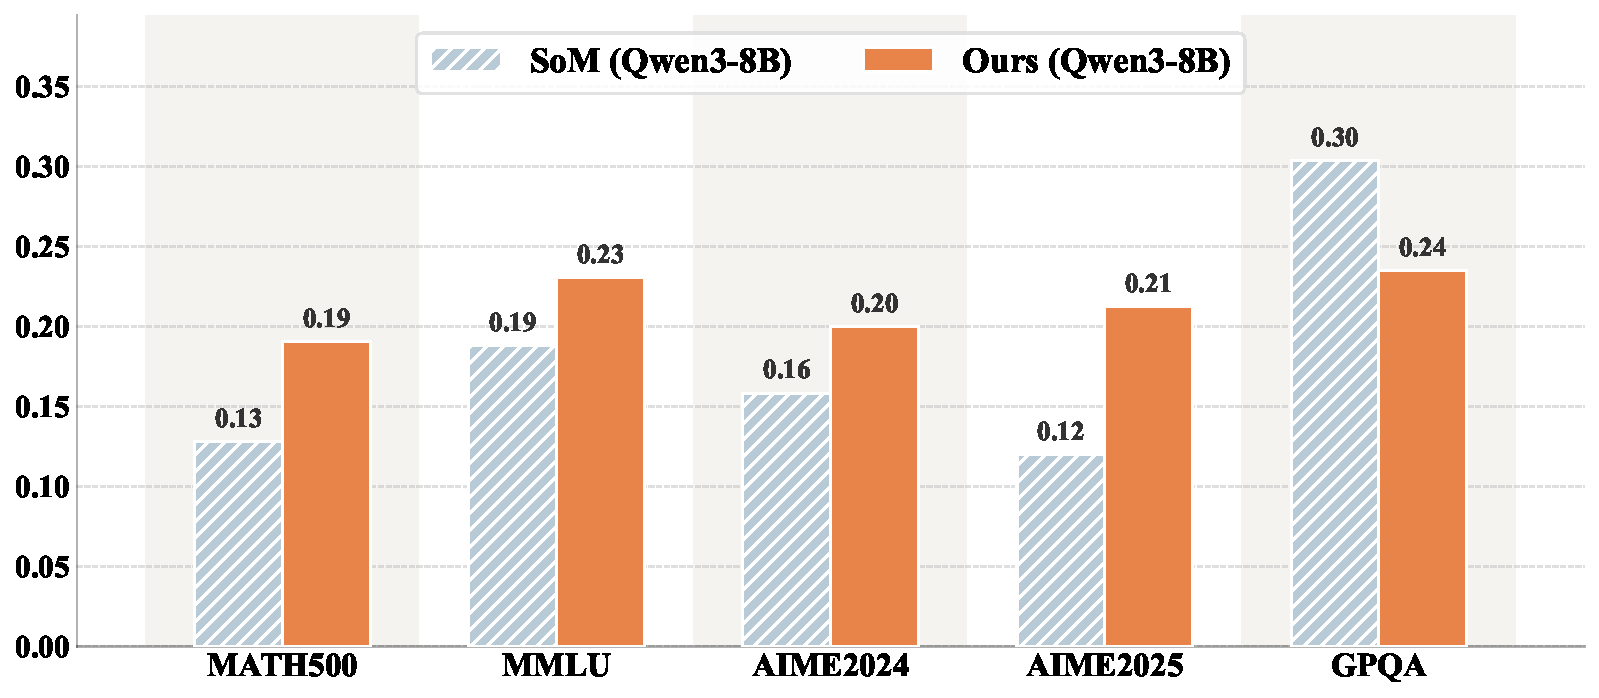
\includegraphics[width=\linewidth]{figures/fig_intra.pdf}
        \caption{Intra-diversity across datasets and backbone models.}
        \label{fig:intra_diversity}
    \end{subfigure}
    \hfill
    \begin{subfigure}[t]{0.495\textwidth}
        \centering
        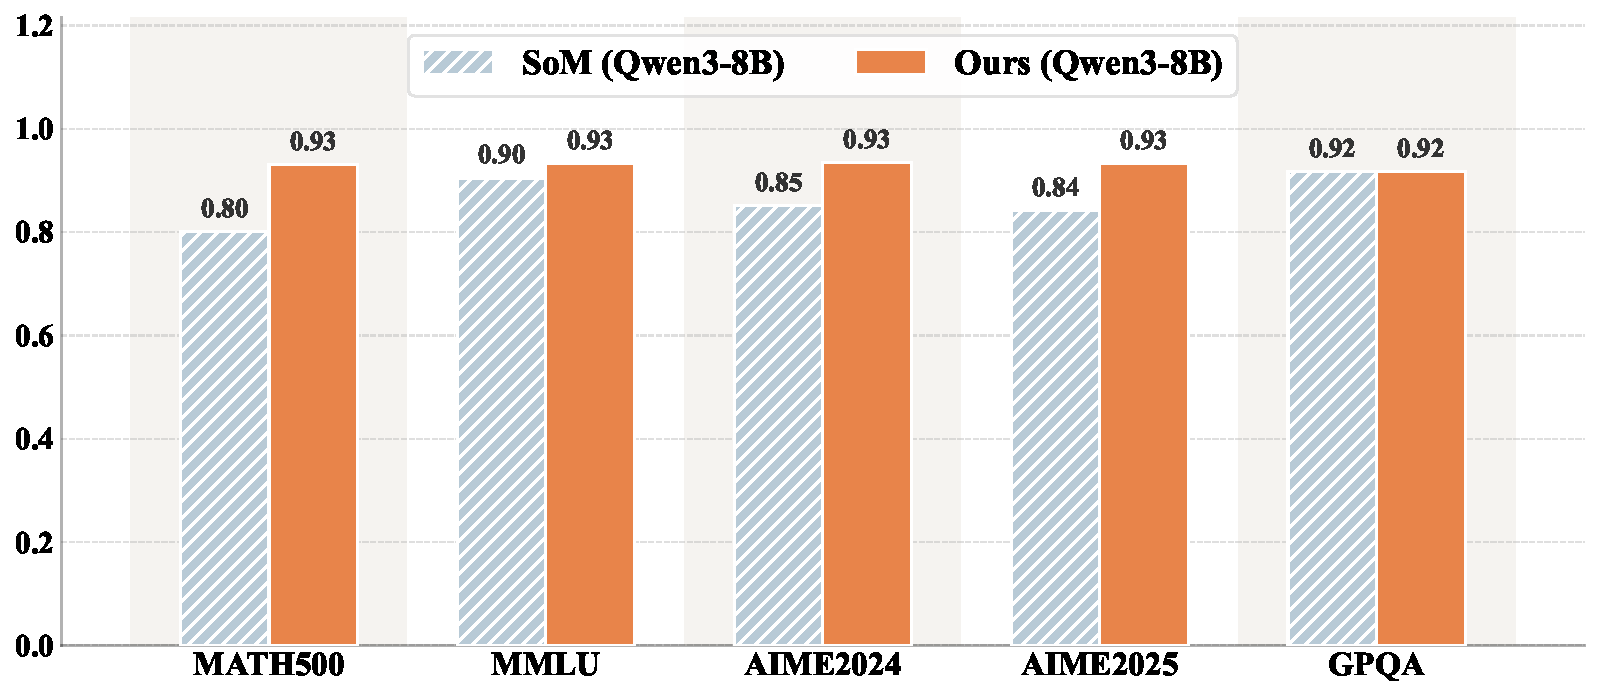
\includegraphics[width=\linewidth]{figures/fig_non_overlap.pdf}
        \caption{Structural non-overlap across datasets and backbone models.}
        \label{fig:structural_nonoverlap}
    \end{subfigure}

    \caption{
    Diversity analysis of multi-agent reasoning.
    (a) Intra-diversity measures semantic variation among agents.
    (b) Structural non-overlap measures diversity at the reasoning-structure level.
    Our method consistently improves both metrics across datasets, indicating structured and effective diversification.
    }
    \label{fig:diversity_analysis}
    \vspace{-4pt}
\end{figure*}


To quantify the diversity of multi-agent reasoning, we consider two complementary metrics: \textbf{Intra-diversity} and \textbf{Structural Non-overlap}, together with task accuracy to assess whether diversity is beneficial rather than noisy.

\paragraph{Intra-diversity.}
Intra-diversity measures semantic variation among agents' reasoning for the same problem. Given the final responses $\{r_1, \dots, r_N\}$ from $N$ agents, we compute the average pairwise cosine distance between their TF--IDF representations:

\begin{equation}
\begin{aligned}
\mathrm{IntraDiv}(x)
&= \frac{2}{N(N-1)} \sum_{i<j} \big(1 \\
&\quad - \cos\big(\phi(r_i), \phi(r_j)\big)\big),
\end{aligned}
\end{equation}
where $\phi(\cdot)$ denotes TF--IDF encoding. Higher values indicate that agents explore more diverse semantic reasoning paths instead of converging to similar explanations.

\paragraph{Structural Non-overlap.}
While semantic diversity captures surface-level variation, it does not necessarily reflect differences in reasoning structure. To address this, we further measure Structural Non-overlap. For each response $r_i$, we segment the reasoning into step-level units $S_i$, and compute their Jaccard overlap:
\begin{equation}
\mathrm{NonOverlap}(x) = 1 - \frac{2}{N(N-1)} \sum_{i<j} \frac{|S_i \cap S_j|}{|S_i \cup S_j|}.
\end{equation}
Higher values indicate that agents rely on distinct reasoning structures rather than paraphrasing similar logic.

As shown in Figure~\ref{fig:intra_diversity}, our method achieves higher intra-diversity across most benchmarks, including MATH500, MMLU, AIME 2024, and AIME 2025. On GPQA, SoM exhibits slightly higher intra-diversity (0.30 vs.\ 0.24), potentially because surface-level response variation on expert-knowledge problems is less constrained by structured path guidance. Overall, these results indicate that the proposed mechanism effectively encourages agents to explore diverse reasoning paths rather than respond homogeneously.

Figure~\ref{fig:structural_nonoverlap} further demonstrates that step non-overlap is consistently improved across most benchmarks, indicating that the increased diversity arises from genuinely different reasoning structures rather than superficial variations. On GPQA, both methods reach the same step non-overlap score (0.92), suggesting that structural diversity gains are most pronounced on tasks requiring extended multi-step derivation. Importantly, these improvements do not come at the expense of task performance, as the overall accuracy remains competitive and, in some cases, even improves.

Together, these results demonstrate that our approach promotes structured and effective diversity in multi-agent reasoning.
To provide concrete insights into how agents correct errors and diversify reasoning paths in practice, we present detailed qualitative case studies in Appendix~\ref{app:case_study}.


\subsubsection{Discussions on Effect of the Number of Agents.}
Figure~\ref{fig:agent_num_ablation} shows a non-monotonic trend: moving from two to three agents yields consistent gains on most benchmarks, while GPQA peaks at two agents, suggesting the model can generate only two high-quality independent paths for this domain. Beyond three agents, performance plateaus or reverses: once agents outnumber valid paths $K$, the round-robin allocation assigns duplicate initializations, and the model cannot reliably produce additional independent alternatives. Three agents thus represents the optimal configuration.


\begin{figure}[t]
    \vspace{-2pt}
    \centering
    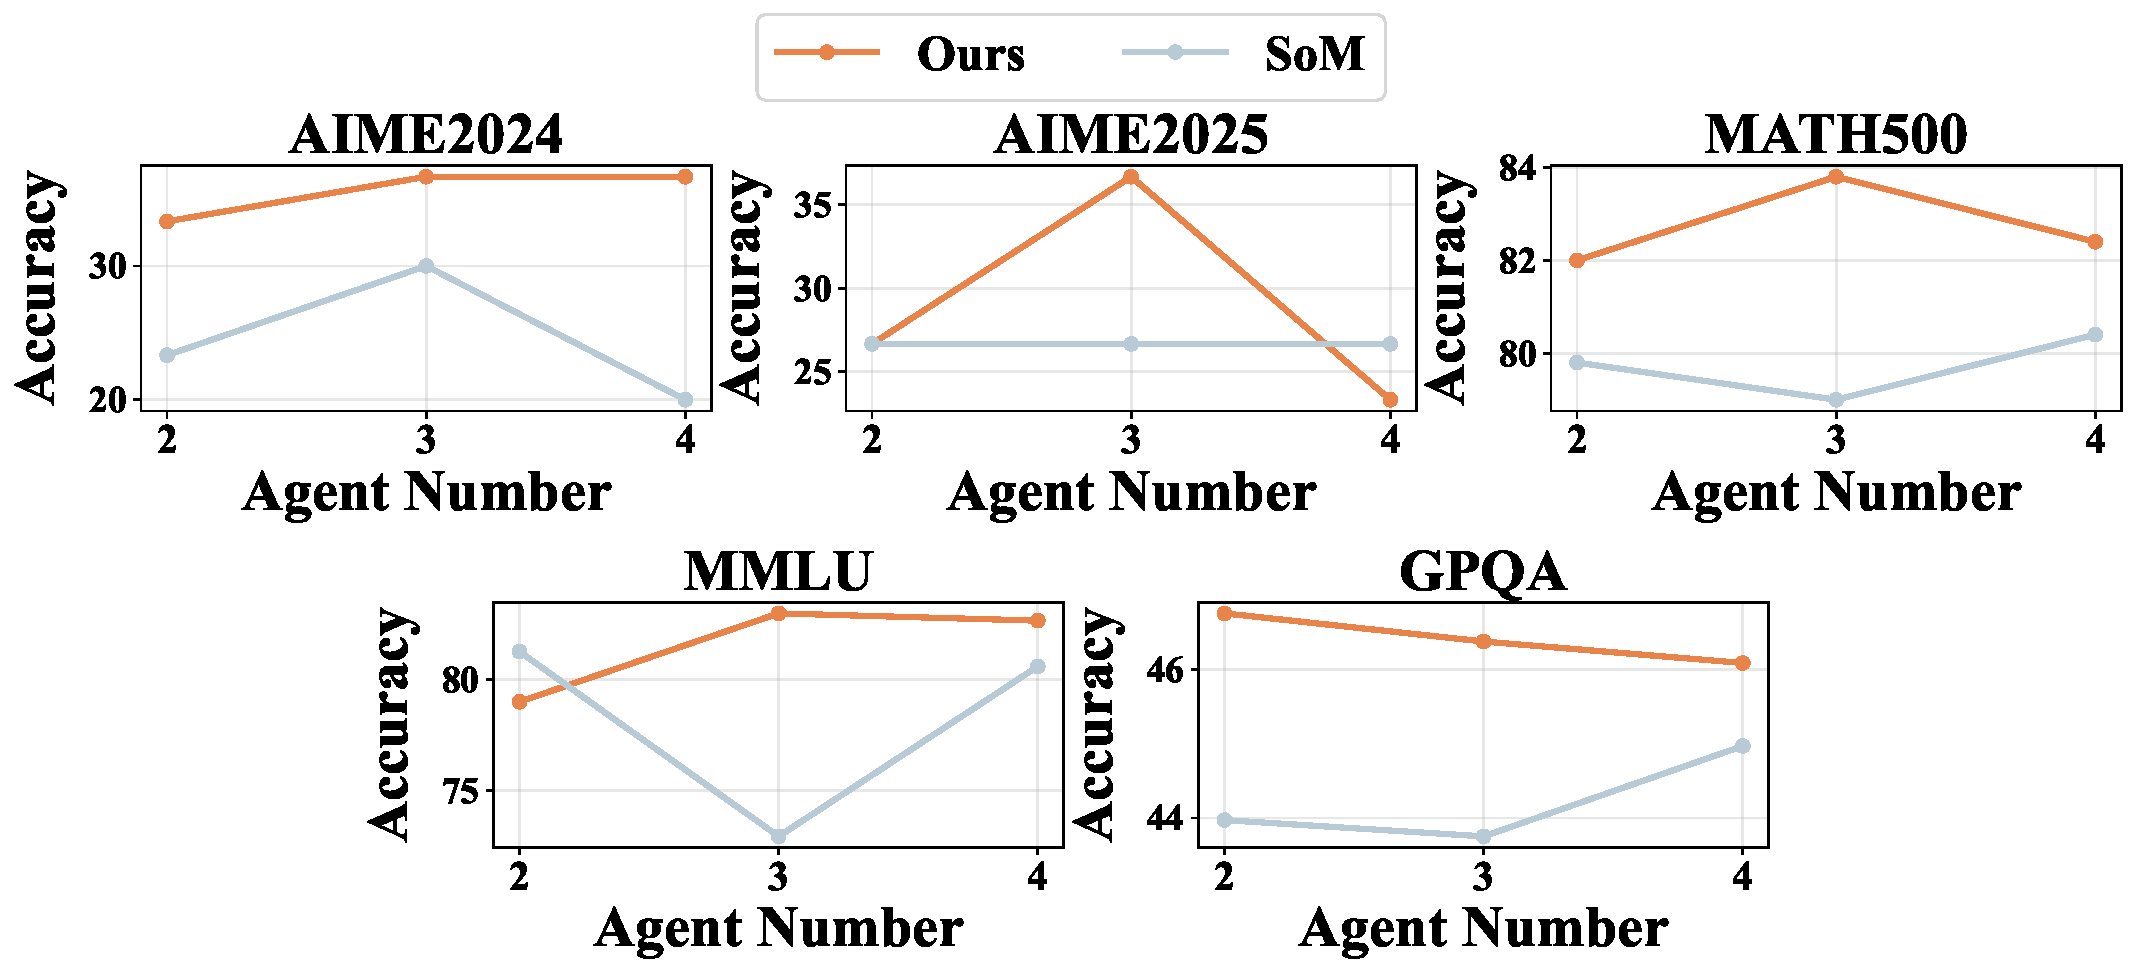
\includegraphics[width=\linewidth]{figures/agent_number_ablation.pdf}
    \caption{Performance comparison under different numbers of agents.}
    \label{fig:agent_num_ablation}
\end{figure}


\subsubsection{Discussions on Effect of Debate Rounds.}
Figure~\ref{fig:round_ablation} shows that hard mathematical tasks peak at Round 2 and degrade at Round 3, as growing context length impairs coherent reasoning and prolonged peer exposure reduces the independence of agent contributions. Knowledge-intensive tasks are more robust, as factual correctness stabilizes once established. Crucially, DynaDebate reaches peak performance by Round 2 on most benchmarks, while SoM requires Round 3 to achieve comparable results—and still falls short—demonstrating that structured initialization enables faster and more efficient convergence.

\begin{figure}[t]
    \vspace{-2pt}
    \centering
    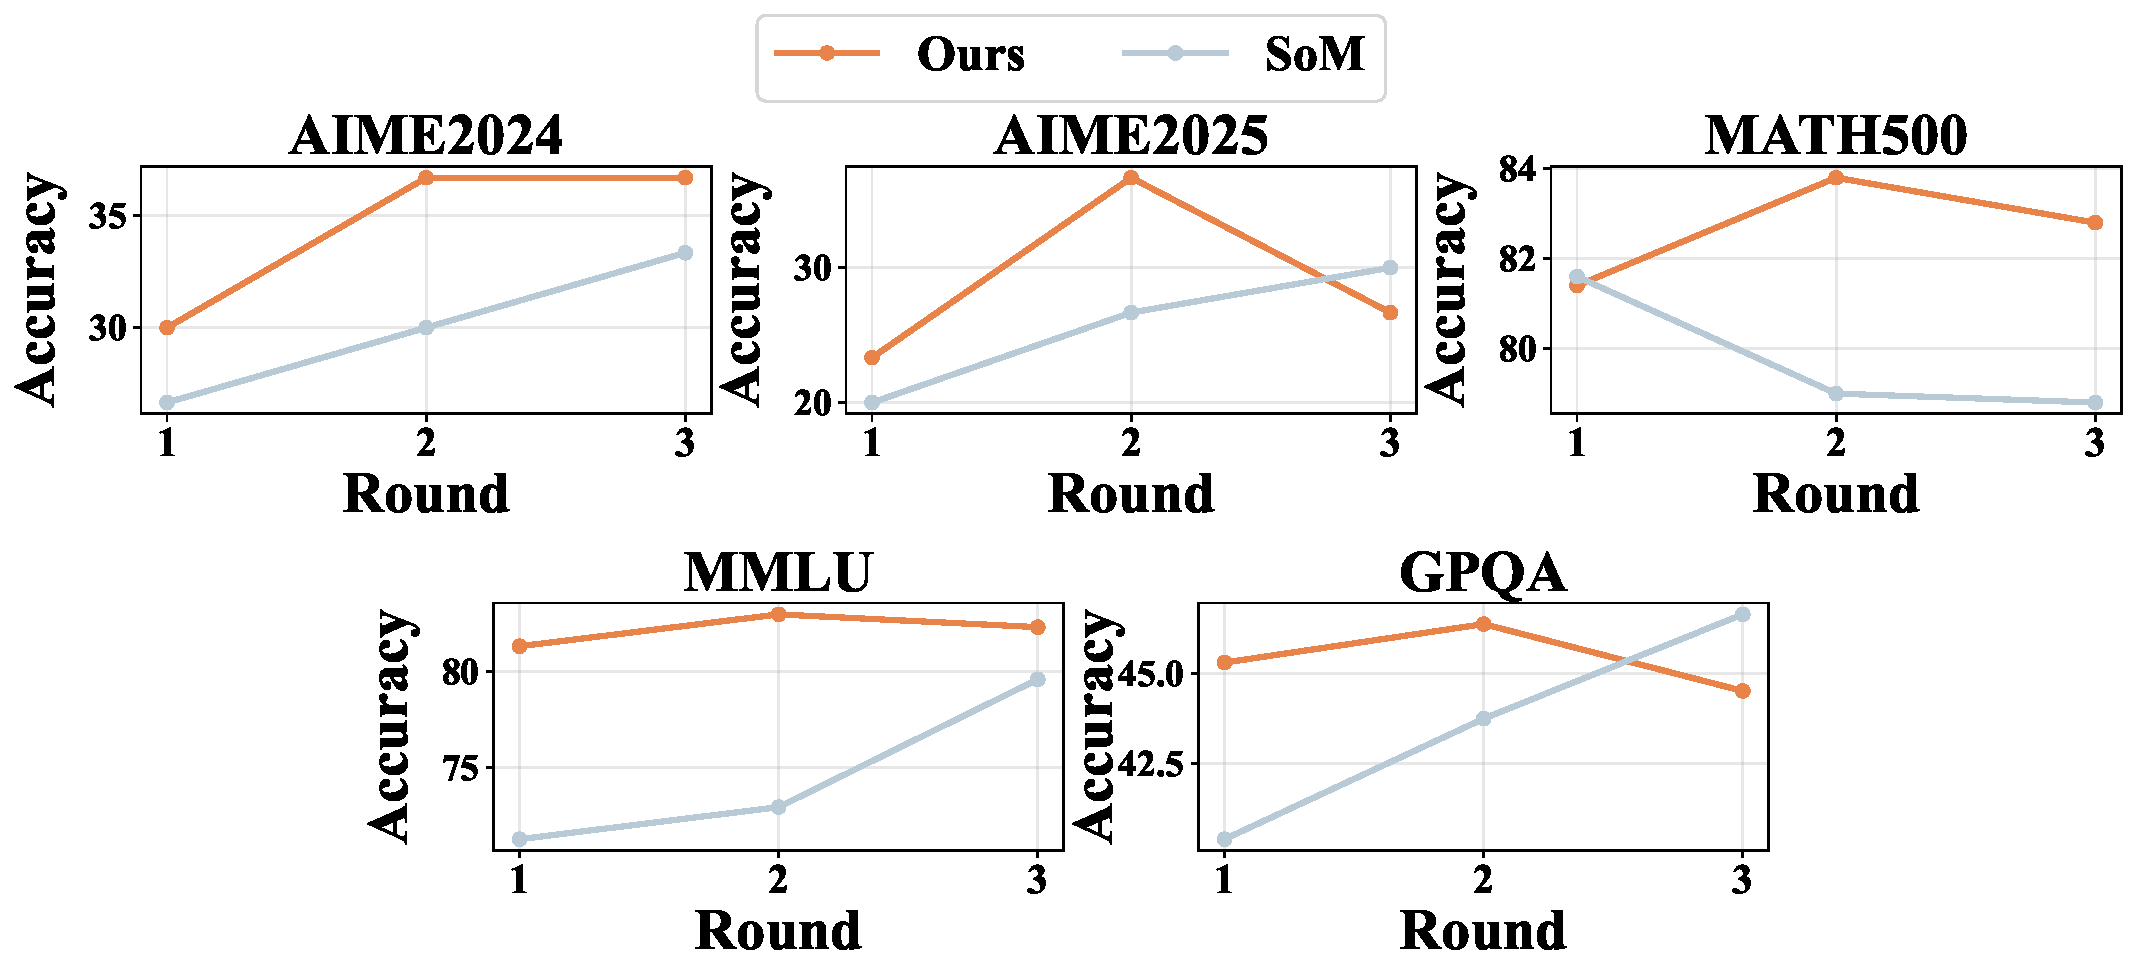
\includegraphics[width=\linewidth]{figures/round_ablation_comparison.pdf}
    \caption{Effect of the number of debate rounds $N$ on performance across benchmarks.}
    \label{fig:round_ablation}
\end{figure}


\subsubsection{Discussions on Computation Cost vs. Performance.}

As shown in Figure~\ref{fig:pareto}, DynaDebate consistently occupies a favorable position on the accuracy--token Pareto frontier, achieving higher accuracy at comparable token budgets relative to all baselines. Moreover, this overhead is selective rather than uniform, as verification triggers predominantly on the hardest problems (Appendix~\ref{app:trigger_stats}). Per-round token costs appear in Appendix~\ref{app:cost}.

\begin{figure}[tb]
    \centering
    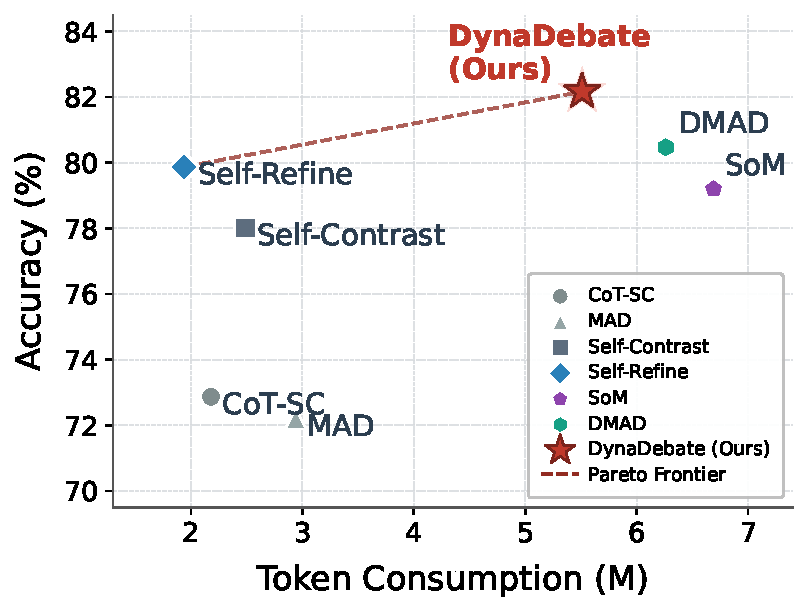
\includegraphics[width=\linewidth]{figures/token_accuracy_pareto.pdf}
    \caption{Accuracy--token Pareto frontier on MATH500. DynaDebate consistently achieves higher accuracy at comparable token budgets relative to baselines.}
    \label{fig:pareto}
\end{figure}
